

\chapter{Présentation}
\label{chap:presentation}
%\minitoc

\section{Introduction}
Dans le cadre de mon cursus universitaire en master MIAGE (méthodes informatiques appliquées à la gestion des entreprises) à l'université Paris Nanterre, je réalise un stage du 09/04/2018 au 24/08/2018 au sein de l'entreprise Tastycloud. Ce stage a pour but de mettre en pratique les aspects théoriques vus en master c'est à dire les processus de modélisation et développement à la réalisation de tâches. Il est donc important que le stage soit en adéquation avec un profil master qui demande au stagiaire de ne plus avoir un simple rôle d'exécutant mais d'être un maillon à part entière dans l'entreprise en participant activement à son développement et en y apportant ses idées et comment les mettre en oeuvre.\\

Ce premier stage du cursus MIAGE est donc un point essentiel pour avoir une première approche réelle de la conception accompagnée de la réflexion dans un milieu professionnel. Il permet également à l'étudiant d’évaluer sa capacité, son adaptabilité, ses connaissances et sa réactivité à différentes situations auxquelles on peut le confronter.\\

C'est donc pourquoi, lors de ma recherche de stage, je me suis orienté vers un stage de développement informatique qui recherchait un profil d'ingénieur (bac plus quatre et plus cinq) qui demandait un esprit analytique, être autonome et responsable dans son travail. J'avais auparavant cherché différents stages dans le développement que ce soit du web ou d'autre domaine mais c'était bel et bien le développement mobile qui m'intéressait le plus. C'est donc tout naturellement que j'ai postulé chez Tastycloud qui proposait un stage Android pour la maintenance de leur logiciel.\\

Ce rapport de stage a pour but de présenter l'entreprise et les différentes missions réalisées. Que propose l'entreprise et quel est sa solution ? En quoi consistait mon travail durant ce stage ? Quels sont les choix qui ont été décidés pour les différentes missions et pourquoi ? Comment ont-elles été mises en oeuvres ?\\

Dans un premier temps je ferai une mise en contexte en présentant l'entreprise de manière générale c'est à dire son secteur d'activité, ses différents pôles, son logiciel et ma place dans cette dernière. Je parlerai ensuite de mes différentes missions de stage les objectifs attendus ainsi que les outils mis à ma disposition pour la réalisation des missions. Enfin j’expliquerai les solutions choisies et adoptées pour résoudre les différents problèmes rencontrés durant le stage. Je préciserai également tout le processus de développement et réflexion qui a été mis en oeuvre. Je conclurai ainsi sur une synthèse de l'apport de mon travail à l'entreprise, ce que j'ai appris à titre professionnel et personnel.

\clearpage


\section{Présentation de l'entreprise}
\subsection{TastyCloud}
Tastycloud est une startup fondée en septembre 2016 spécialisée dans le digital. L'idée est d'apporter aux restaurateurs une solution de tablettes numériques qui viendraient remplacer le menu papier. L'objectif de cette solution est de donner aux restaurateurs un moyen de mieux gérer leur carte et d'augmenter leur chiffre d'affaire. Cette augmentation du chiffre d'affaire passe par des fonctionnalités du logiciel qui pousse et oriente le l'utilisateur dans sa consommation. La société a su, depuis 2016, se développer en mettant en place sa charte graphique, son business plan puis en trouvant ses premiers clients en 2017. Elle est aujourd'hui une des sociétés les plus importantes du marché des tablettes tactiles dans les restaurants.\\

Les clients de Tastycloud se trouvent un peu partout en France. Au départ la société se limitait à des restaurants parisiens mais aujourd'hui elle se développe dans le sud de la France, les Alpes, en Bretagne, dans le Jura etc... Tastycloud a pour objectif de s'exporter à l'international dans le futur et conquérir de nouveaux marchés.\\

Tastycloud possède aujourd'hui son siège à Paris plus précisément dans le 15ème arrondissement près de porte de Versailles. Cela n'empêche pas l'équipe d'être polyvalente et itinérante et de se déplacer pour leurs clients et pour les salons.


\subsection{L'entreprise en quelques chiffres}

\begin{figure}[!htb]
  \centering
  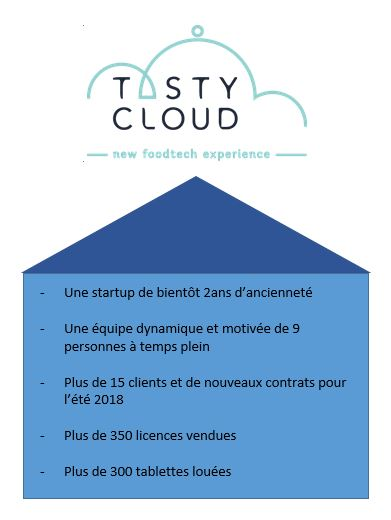
\includegraphics[width=75mm,scale=0.5]{tastystat.JPG}
  \caption{Les chiffres de l'entreprise}
  \label{fig:boat1}
\end{figure}

\subsection{Fonctionnement de l'entreprise}

Tastycloud est une solution clé-en-main. En plus du logiciel sur tablette, l'entreprise fournit divers services tels que :

- L'écoute du besoin client et le développement de fonctionnalités suivant leurs besoins. Le client est constamment mis à contribution dans l'évolution de la solution et le processus de développement étant une partie prenante importante.

- Configuration de la carte à l'aide d'un back office (qui sera présenté plus tard) côté restaurateur qui lui permet de gérer sa carte. Il peut rajouter des produits des formules, des conditions (carte du midi, carte du soir), des options. Ce back office permet aussi au restaurateur d'avoir des statistiques sur ses ventes et les consultations des clients.

- Photographie professionnelle des plats, un photographe professionnel est dépêché sur place pour shooter la totalité de la carte. Bien sûr cela est facultatif si le restaurateur veut prendre ses photos lui-même.

- Traductions des menus,. Comme pour les photos, des professionnels traduisent les menus selon les langues choisies par le client.

- Installation de la solution dans le restaurant (tablettes, espace de rechargement, paramétrage et formation).

- Mise à jour automatique du logiciel lors de la mise en production de nouvelles fonctionnalités.

- L'hébergement des données et data sur le cloud

Tastycloud fournit aussi une assistance aux restaurants toute la semaine et le week-end si besoin ainsi que des assurances vol et casse sur les tablettes. Le service est facturé à 1,50\euro/jour par tablette. Il y a aussi des frais d'installation.
La startup compte beaucoup sur son réseau et les salons autour du foodtech et digital pour trouver de nouveaux clients. Elle s'adonne aussi à la prospection à Paris et à la communication sur les réseaux sociaux.

\subsection{Le logiciel}

Pour bien comprendre de quoi nous parlons, faisons une petite présentation du logiciel d'un point de vue client :

\begin{figure}[!htb]
  \centering
  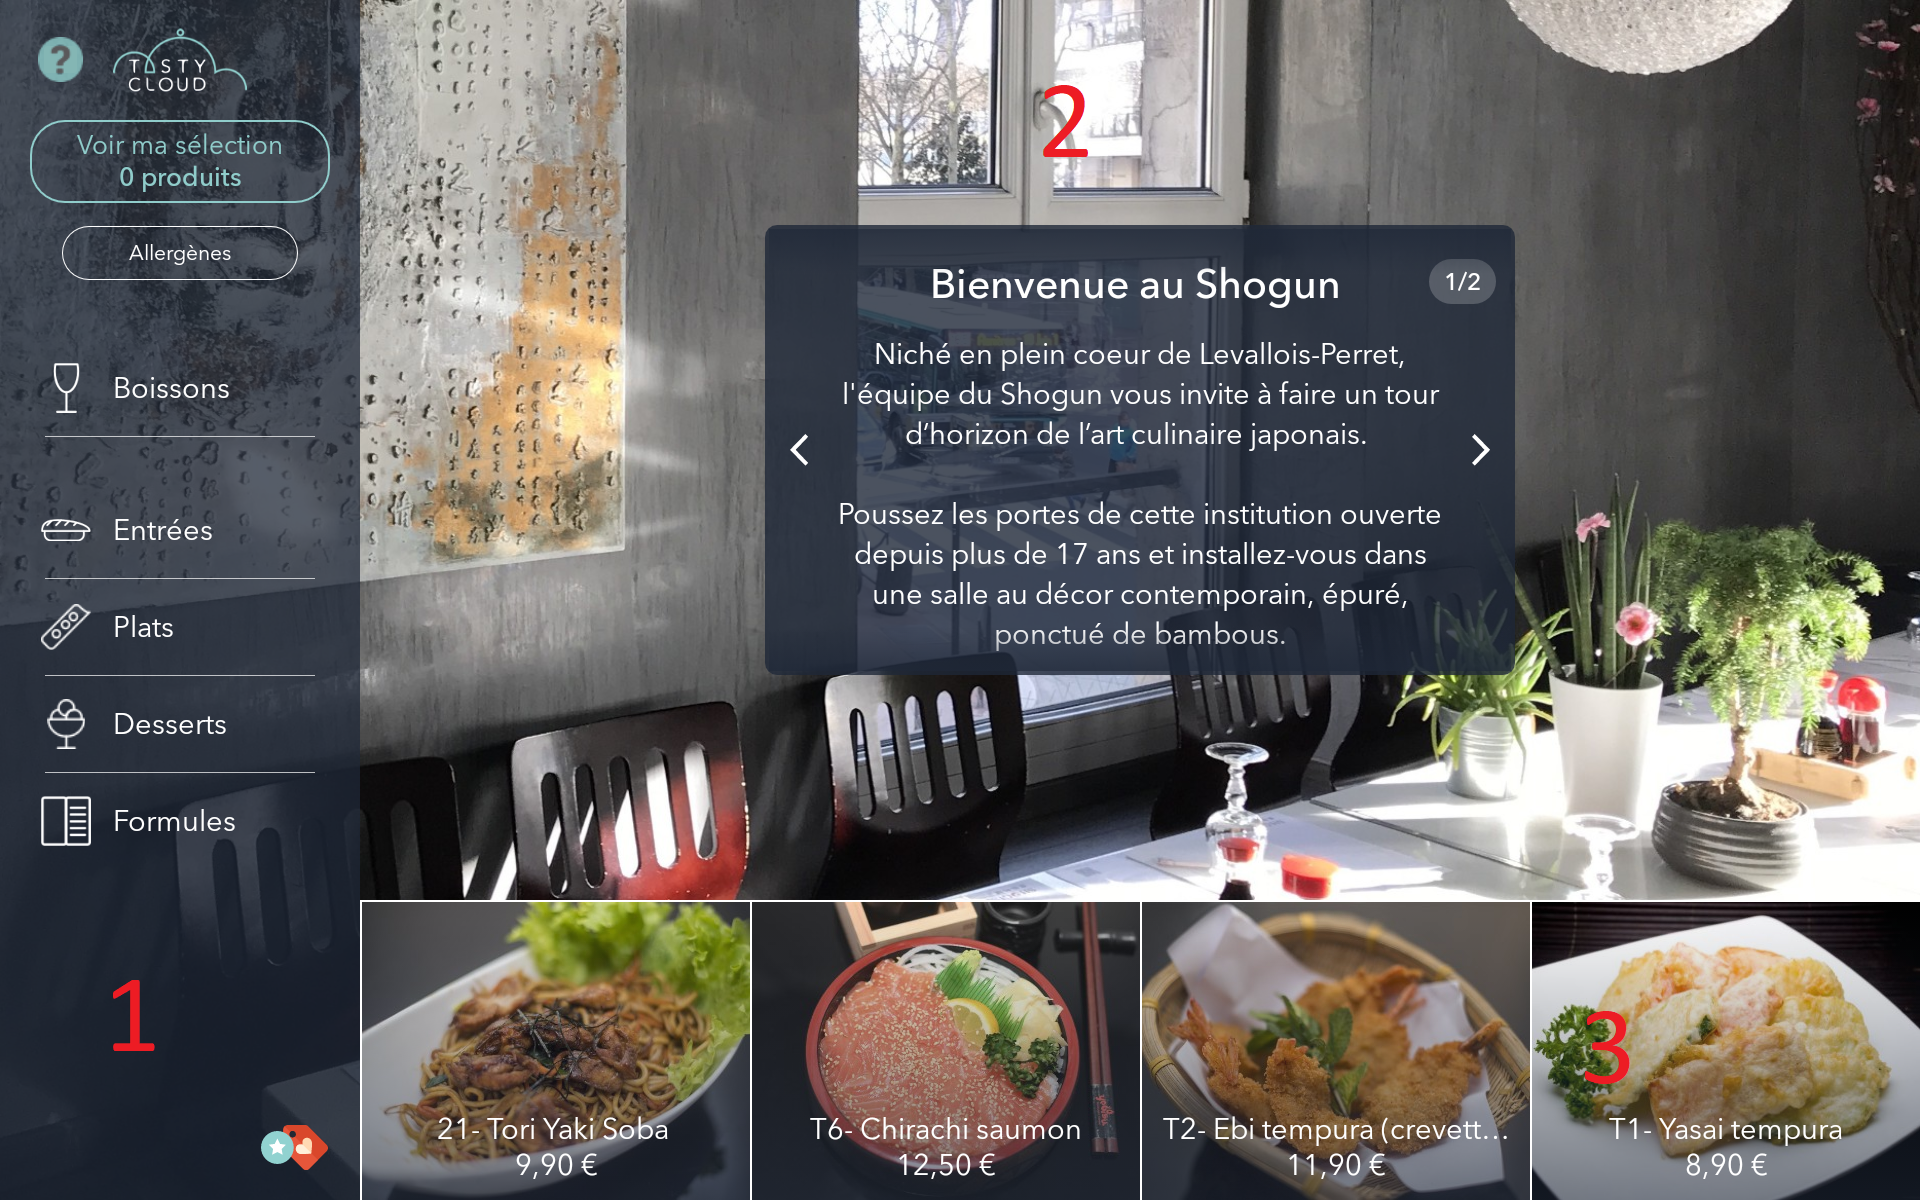
\includegraphics[width=105mm,scale=0.5]{home_tastycloud.png}
  \caption{Le menu "Home" de l'application}
  \label{fig:boat1}
\end{figure}

Voici la page d'accueil d'un restaurant (ici le Shogun). C'est la première page sur laquelle tombe le client. Si nous décomposons l'accueil en 3 rectangles délimités sur la capture d'écran par les numéros un, deux, trois en rouge nous pouvons dire que :

- Le 1 désigne le menu sur lequel le client peut aller chercher ses produits, ses formules ou sa sélection. Comme nous pouvons le voir les produits sont classés par type (boissons, entrées ...). Nous pouvons aussi avoir le choix des langues en bas à gauche mais cette option n'est pas disponible sur ce restaurant. Il y a aussi une option pour les allergènes qui est normalement obligatoire dans les restaurants. La sélection et les allergènes s'ouvrent dans des pop-ups. Pour ce qui est du bouton en haut à gauche il s'agit d'une fonctionnalité que j'ai moi-même développée et nous aurons par conséquent l'occasion de voir tout ça ultérieurement.

- Le 2 est une page de présentation, c'est sur ce rectangle et le 3 que les sous menus vont s'ouvrir (visible sur la capture d'écran ci-dessous) et que l'on va pouvoir naviguer dans l'application.

- Le 3 représente les suggestions de l'établissement, c'est le restaurateur qui choisit les produits qu'il veut mettre en avant sur sa page d'accueil pour avoir une meilleure visibilité des clients.

\begin{figure}[!htb]
  \centering
  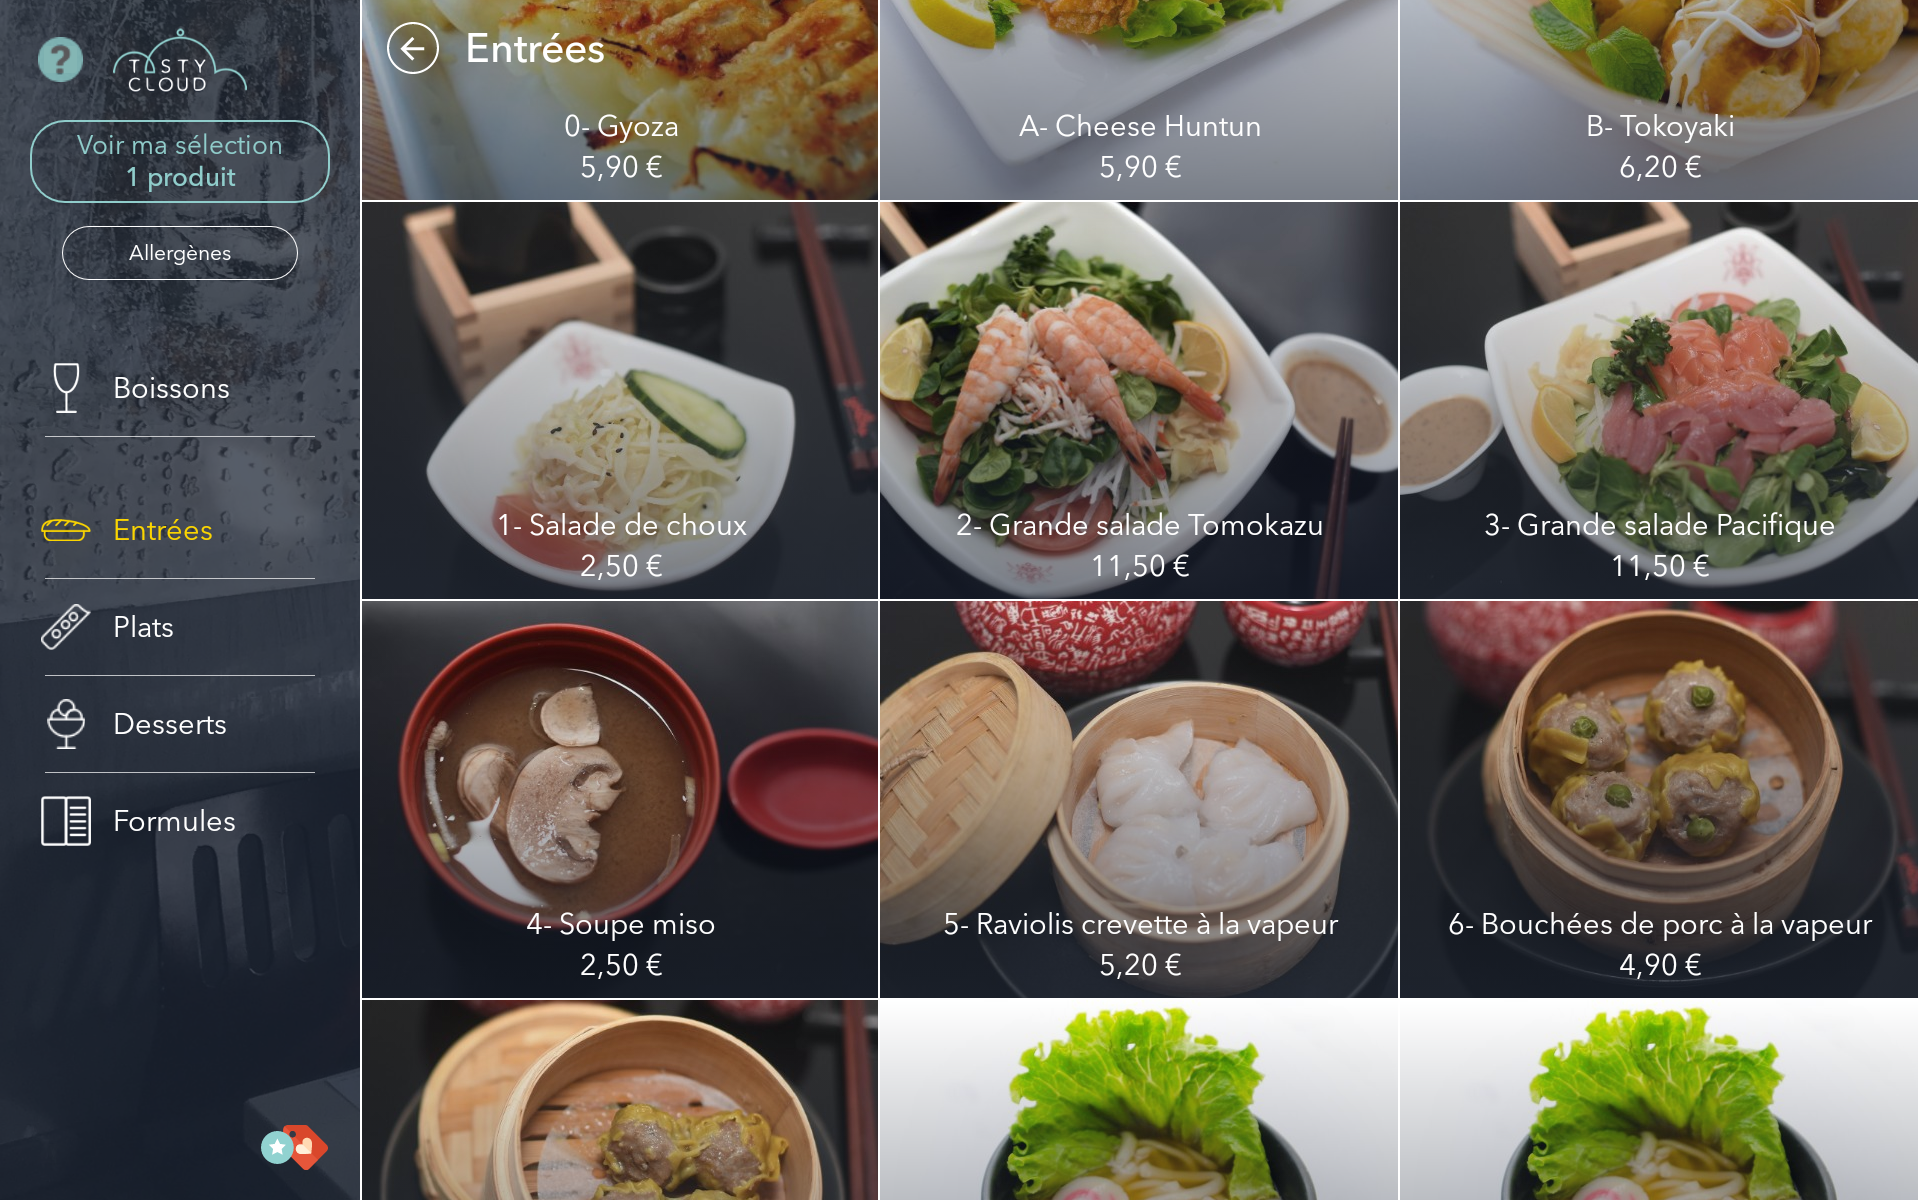
\includegraphics[width=105mm,scale=0.5]{entree_tastycloud.png}
  \caption{Ouverture du menu "Entrées" sur l'application}
  \label{fig:boat1}
\end{figure}

\subsection{Mon poste de travail}

J'ai donc effectué mon stage au siège de Tastycloud dans le 15ème arrondissement à Paris. La société est composée de plusieurs pôles : technique, commercial, opérationnel et marketing. J'ai logiquement travaillé dans le pôle technique avec mon tuteur et d'autres stagiaires. C'est le plus important en terme d'effectifs. L'application grandissant de jour en jour il faut de plus en plus de personnes pour la maintenir (Que ce soit le logiciel ou le back office).\\

L'organisation du bureau est dite en "OpenSpace" ce qui favorise la communication entre les différents membres de l'équipe et qui a pour conséquence d’augmenter la créativité, favoriser l’efficacité au résultat, l'échange d'idées et les suggestions selon les différents points de vue de la startup.

%%% Local Variables: 
%%% mode: latex
%%% TeX-master: "isae-report-template"
%%% End: 
